

\documentclass[11pt]{article}
\usepackage[utf8]{inputenc}
\usepackage{geometry}
\usepackage{graphicx}
\usepackage{hyperref}
\usepackage{amsmath}
\usepackage{listings}
\usepackage{xcolor}
\usepackage{float}
\usepackage{subcaption}
\usepackage{algorithm}
\usepackage{algpseudocode}
% Set page margins
\geometry{a4paper, margin=1in}

% Set up code listing style
\lstset{
    basicstyle=\ttfamily,
    commentstyle=\color{gray},
    keywordstyle=\color{blue},
    stringstyle=\color{red},
    showstringspaces=false,
    captionpos=b
}

\title{Diffusion models: M2 coursework report}
\author{Vishal Jain}
\date{\today}

\begin{document}

\maketitle

\tableofcontents

\newpage
% TODO: Make bold vectors consistent. Use \mathbf{} for all vectors.
\section{Introduction - Denoising Diffusion Probabilistic Models}
\subsection{Model Architecture}
The denoising diffusion probabilistic model (ddpm) consists of an encoder and decoder.
The encoder is predetermined and defines the forward degradation process. The decoder is learnt and describes the denoising process. All the learnt parameters associated with the ddpm model are in the decoder network.
\subsubsection{Encoder}
The encoder takes as input an image $x$ and outputs a latent (degraded) representation $z$ through some degradation process. The implementation of the ddpm encoder in the original notebook degrades the input image $x$ by gradually adding gaussian noise $\epsilon$ at each step $t$. It follows an update scheme:
\begin{equation}
    \begin{aligned}
        z_1 &= \sqrt{1-\beta_1} \cdot x + \sqrt{\beta_1} \cdot \epsilon_1 \\
        z_t &= \sqrt{1-\beta_t} \cdot z_{t-1} + \sqrt{\beta_t} \cdot \epsilon_t \quad \forall t \in 2, \ldots, T,
    \end{aligned}
    \end{equation}
    where $\epsilon_t \sim \mathcal{N}(0, I)$, $\beta_t \in [0,1]$ is the noise schedule, $T$ is the total number of steps and $z_t$ describes the latent representation at step $t$.

This is equivalent to the following update rule which can be used to calculate the latent variable $z_t$ directly from $x$:
\begin{equation}
    z_t = \sqrt{\alpha_t} \cdot x + \sqrt{1 - \alpha_t} \cdot \epsilon, \quad \text{where } \alpha_t = \prod_{s=1}^{t} (1 - \beta_s).
    \label{eq:z_t_alpha}
\end{equation}

The implementation in the notebook uses the following linear schedule for $\beta_t$:
\begin{equation}
    \beta_t = \frac{t}{T}(\beta_{max}-\beta_{min})+ \beta_{min},
\end{equation}
where the default values are $\beta_{max} = 0.02$, $\beta_{min} = 0.0001$ and $T=1000$.

\subsubsection{Decoder}
The decoder takes as input a latent representation (noisy image) $z$, the current time step $\frac{t}{T}$ and outputs the noise which can be used to obtain the denoised image. The default decoder network in the notebook is structured as a convolutional neural network (CNN) with 5 layers, each configured to preserve the spatial dimensions of its input through the application of zero padding. The network architecture specifies a progression of feature channels as follows: it starts with an input of 1 channel, then expands to 16 channels in the first layer, increases to 32 channels through the second and third layers, contracts back to 16 channels in the fourth layer, and finally reduces to 1 channel in the fifth output layer. The first four convolutional layers use a 7x7 kernel size, while the final convolutional layer employs a 3x3 kernel, with all layers using a GELU activation function.

The decoder network also includes a fully connected network to calculate the time encodings, which is a high-dimensional representation of the scalar time step $\frac{t}{T}$. This involves generating a set of exponentially increasing frequencies to capture patterns at various scales, computing the sine and cosine for each time step across all frequencies to provide a cyclic representation of time that captures periodic patterns, and concatenating these sine and cosine values to form a unique time signature. This signature is then transformed through multiple linear layers, creating a high-dimensional representation of the scalar time step. This vector is reshaped so it can be broadcasted across the spatial domain of the feature map of the first layer in the CNN when added to it. This process effectively "informs" each spatial location in the feature maps about the current stage of the diffusion process, allowing the network to undo the appropriate amount of noise at each stage. The specific network used to learn the time encoding is a multi layer perceptron (MLP) with 2 hidden layers with 128 hidden units in each, the input layer takes the concatenated sine and cosine tensor of shape 32 (16*2) and the final layer outputs a tensor of size 16 - the number of channels output by the first convolutional layer in the CNN. All layers use a GELU activation function.

\subsection{Training Algorithm}
The optimal model parameters $\phi$ for the decoder network are by found by maximising the log likelihood of the training data $\{x_i\}_{i=1}^{I}$:

$$\hat{\boldsymbol{\phi}} = \arg\max_{\boldsymbol{\phi}} \left[ \sum_{i=1}^{I} \log \Pr(x_i | \boldsymbol{\phi}) \right] \quad$$

This is approximately equivalent to minimising the following loss function:
$$
L[\boldsymbol{\phi}] = \sum_{i=1}^{I} \sum_{t=1}^{T} \left\| g[\mathbf{z}_{it}, \frac{t}{T}; \boldsymbol{\phi}] - \boldsymbol{\epsilon}_{it} \right\|^2
$$
\begin{equation}
= \sum_{i=1}^{I} \sum_{t=1}^{T} \left\| g \left[\sqrt{\alpha_t} \cdot \mathbf{x}_i + \sqrt{1 - \alpha_t} \cdot \boldsymbol{\epsilon}_{it}, \frac{t}{T}; \boldsymbol{\phi} \right] - \boldsymbol{\epsilon}_{it} \right\|^2,
\label{eq:loss_function}
\end{equation}

where $g$ is the decoder network.

The training algorithm works as follows: Loop over all batches in the current epoch, for every image in the batch randomly sample the current time step $t$ from a uniform distribution over the interval $[1, T]$. Then sample the noise $\boldsymbol{\epsilon}$ from a standard normal distribution. The latent representation $\boldsymbol{\mathbf{z}}_{t}$ is then calculated using the update rule given in equation \eqref{eq:z_t_alpha}. Input the latent variable $\boldsymbol{\mathbf{z}}_{t}$ and the time step fraction $\frac{t}{T}$ into the decoder network which then outputs the noise estimate $\hat{\boldsymbol{\epsilon}}$. Calculate the mean square error between the estimated noise and the true noise. Accumulate the losses over the entire batch and take a gradient step using the ADAM optimiser. Repeat for several epochs. This process is described in the pseudocode below:

\begin{algorithm}
\caption{Diffusion model training}
\begin{algorithmic}[1]
\State \textbf{Input:} Training data $x$
\State \textbf{Output:} Model parameters $\boldsymbol{\phi}$
\While{not converged} \Comment{Repeat until convergence}
    \For{$i \in \mathcal{B}$} \Comment{For every training example index in batch}
        \State $t \sim \text{Uniform}[1, \ldots, T]$ \Comment{Sample random timestep}
        \State $\boldsymbol{\epsilon} \sim \text{Norm}[0, \mathbf{I}]$ \Comment{Sample noise}
        \State $\boldsymbol{\mathbf{z}}_{t} = \sqrt{\alpha_t} \cdot \mathbf{x}_i + \sqrt{1 - \alpha_t} \cdot \boldsymbol{\epsilon}$ \Comment{Calculate latent variable}
        \State $\hat{\boldsymbol{\epsilon}} = g_t \left( \boldsymbol{\mathbf{z}}_{t}, \frac{t}{T}; \boldsymbol{\phi}_t \right)$ \Comment{Estimate the noise}
        \State $\ell_i = \left\|\hat{\boldsymbol{\epsilon}} - \boldsymbol{\epsilon} \right\|^2$ \Comment{Compute individual loss}
    \EndFor
    \State Accumulate losses for batch and take gradient step
\EndWhile
\end{algorithmic}
\end{algorithm}
\section{Training}
In this section the training of the default diffusion model is documented for 2 different sets of hyper parameters.
\subsection{Choice of Hyperparameters}
To demonstrate some of the underlying assumptions behind diffusion models, the following runs vary the noise schedule.
Specifically, a constant noise schedule is used where $\beta_t = C, \ \forall t \in \{1,2,...,T\}$, where $C$ is a constant.
The value of C and the total number of steps $T$ are varied between runs. The first run uses a small value of $C$ and a large value of $T$, while the second run uses a large value of $C$ and a smaller value of $T$. The first run is expected to perform better as only a small amount of noise at each step. This is significant because one of the assumptions used to derive the loss defined by \ref{eq:loss_function} is that the reverse distributions $Pr(z_{t-1}|z_{t})$ are well approximated by a normal distribution. This approximation is only valid for small $\beta_t$.
\subsubsection{Training and Validation Loss Curves}
Figure \ref{fig:q1b_loss_curves} shows the training and validation loss curves for the two runs. The first run has a smaller value of $C$ and a larger value of $T$, while the second run has a larger value of $C$ and a smaller value of $T$. The training loss curves for both runs are similar, with the loss decreasing rapidly at the start and then plateauing. The validation loss curves for both runs are also similar, with the loss decreasing rapidly at the start and then plateauing. The validation loss for the first run is lower than the second run, indicating that the first run has a better model. This is consistent with the expectation that a smaller value of $C$ and a larger value of $T$ would result in a better model.

\begin{figure}[ht]
    \centering
    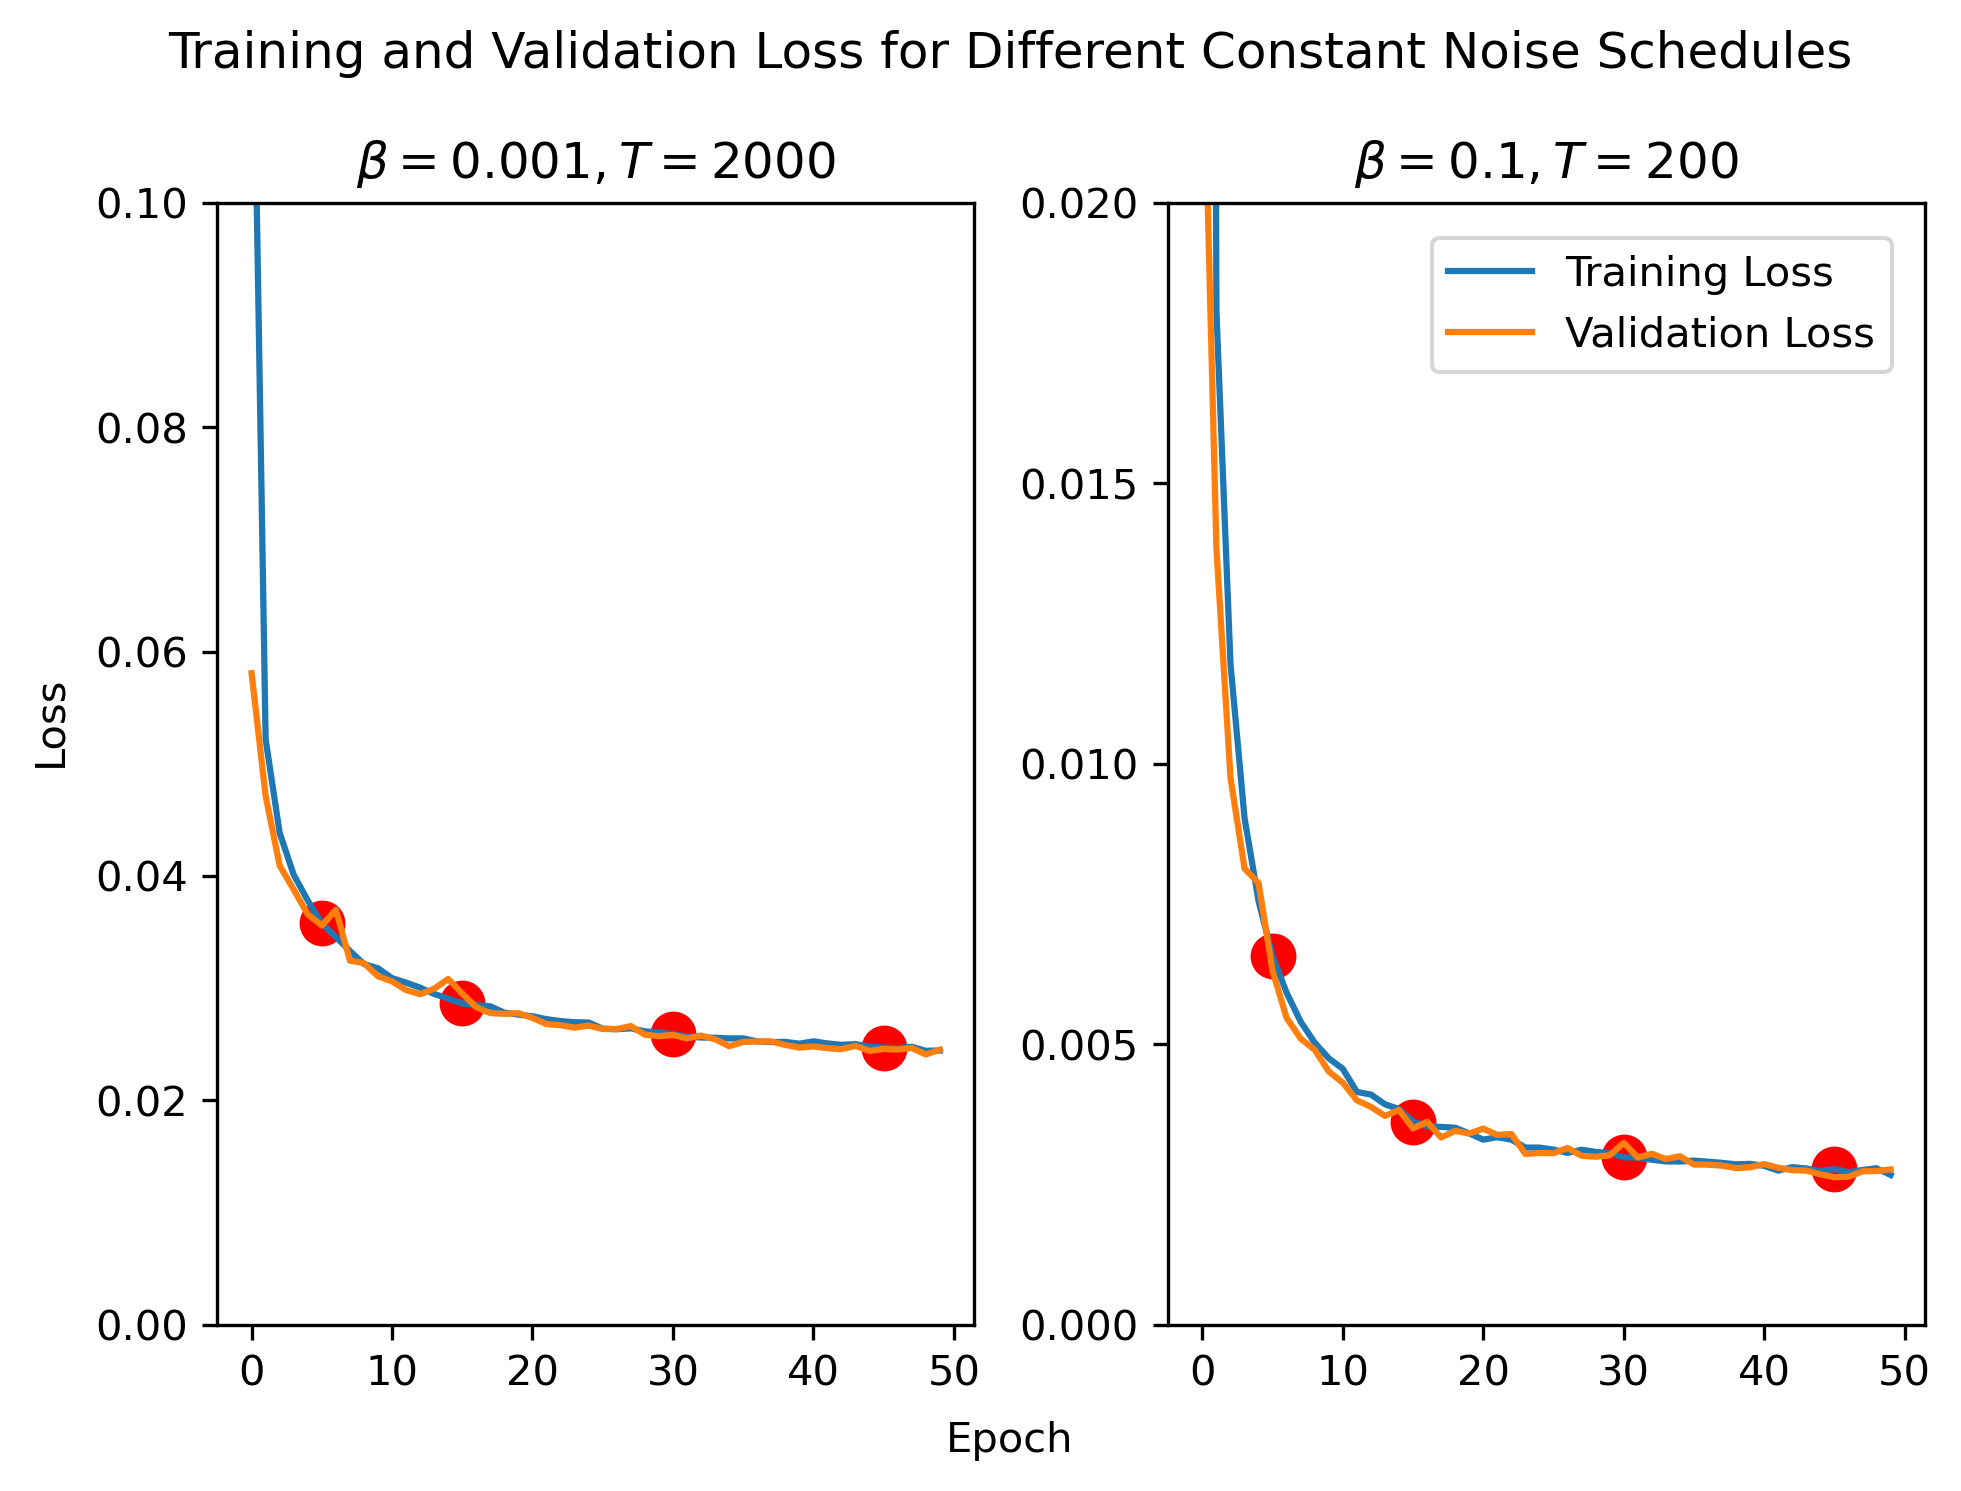
\includegraphics[width=0.8\textwidth]{figs/q1b_loss.png}
    \caption{Description of the figure.}
    \label{fig:q1b_loss_curves}
\end{figure}

\subsubsection{Quality of samples}
Show conditional generation and uncondtional generation 3 different epochs

\section{Evaluation}

\subsection{Discussion of differences}



\end{document}


\end{document}
